\chapter{Solution Design}

This chapter aims to fully describe the solution design from a top to bottom approach. First of all, the general idea of the design is described, abstracting every detail to easily understand the whole. Later on, the different sections of the design are explained with all their characteristics described. The implementation details are left for the following chapters, whereas here we only focus on the ideas and methods used.

In short, the solution to the problem of studying what an observer near a black hole would see is a ray tracer, that is, a device that computes the origin of the rays of light that arrives to a virtual camera placed in a virtual universe.

This work implements a general relativity ray tracer; \ie, a ray tracer for which the path followed by light is not always a straight line.

\section{General Description}

Imagine a spacetime defined by a Kerr metric, with a black hole on its centre, and a camera with a digital sensor placed near it.

As we have studied, all rays that hit the sensor have followed a geodesic to finally arrive to the camera, and their paths are of great interest for us: the origin of the ray will tell us what the particular pixels see and the curvature of the geodesic will let us understand the geometric nature of the spacetime.

For every pixel on the sensor, the ray tracer work can be abstracted as a function that computes the path of the ray that hit it. Therefore, from the pixel coordinates, $p = (p_x, p_y)$, it computes the geodesic path followed by the ray.

This point is computed using the \ac{ODE} system described in \autoref{theo:eqsmotion}, derived from the Kerr spacetime. Therefore, a numerical solver for such systems is needed, along with the initial conditions of each ray. This conforms an \emph{initial value problem}, a kind of well-known problems whose numerical solutions are widely studied.

Abstracting all these tasks out, the general outline of the ray tracer is described on \autoref{alg:raytracer}.

\begin{algorithm}
	\caption{High-level abstraction of the ray tracer}
	\label{alg:raytracer}
	\begin{algorithmic}[1]
		\Function{Ray Tracer}{}
		\State ODEsystem $\gets$ Geodesics equations for the Kerr spacetime
		\State Camera $\gets$ Pinhole camera model
		\State Geodesics $\gets \{\emptyset\}$
		\For{pixel $p = (p_x, p_y)$ in the Camera sensor}
			\State initCond $\gets$ initConditions($p_x$, $p_y$)
			\State $\gamma_{xy} \gets$ solveInitValueProblem(ODEsystem, initCond)
			\State Geodesics $\gets$ Geodesics $\cup$ $\gamma_{xy}$
		\EndFor
		\Return{Geodesics}
	\EndFunction
	\end{algorithmic}
\end{algorithm}

The solution designed for the ray tracer is based on the algorithm described in \cite{thorne15}, that assumes the following:
\begin{enumerate}
	\item The spacetime is defined by the Kerr metric written in Boyer-Lindquist coordinates (see \autoref{eq:kerrmetric}), with a black hole in the centre of the spatial coordinates parametrized by its spin $a$. Its mass is assumed to be 1.
	\item The \ac{FIDO} is a locally non-rotating observer. We define a family of \ac{FIDO} at rest in space with orthonormal basis vectors $\{e_{\widehat{r}}, e_{\widehat{\vartheta}}, e_{\widehat{\varphi}}\}$, pointing along the spatial coordinate lines.
	\item A camera is placed outside of the horizon of the black hole.
	\begin{enumerate}
		\item The position of the camera is described by the coordinates $\{r_c, \vartheta_c, \varphi_c\}$.
		\item The camera speed with respect to the \ac{FIDO} is noted as $\beta$.
		\item The direction of motion relative to the \ac{FIDO} is described by a unit vector $B$ in the camera's reference frame.
		\item We set up a right-handed coordinate system placed on the camera's reference frame, with the orthonormal basis $\{e_x, e_y, e_z\}$, where
		\begin{itemize}
			\item $e_y$ is identified with $B$, \ie, it points to the direction of motion of the camera.
			\item $e_x$ is perpendicular to $e_y$ and contained on the plane $\langle e_{\widehat{r}}, e_{\widehat{\vartheta}} \rangle$.
			\item $e_z$ is perpendicular to $e_x$ and to $e_y$.
		\end{itemize}
		\item We set up a spherical coordinate system derived from the previous one, noted as $\{\vartheta_{cs}, \varphi_{cs}\}$, where:
		\begin{itemize}
			\item $\vartheta$ is the polar angle with respect to the coordinate system origin.
			\item $\varphi$ is the azimuthal angle with respect to the coordinate system origin. The black hole is assumed to rotate in the positive $\varphi$ direction.
		\end{itemize}
	\end{enumerate}
\end{enumerate}

The algorithm consider a set of timelike geodesics arriving at the camera. These geodesics are then integrated backwards to obtain the ray's point of origin on the celestial sphere (at $r = \infty$). These points are noted as $(\vartheta', \varphi')$.

In short, the algorithm goal is to compute the following map
\begin{equation}
	\label{eq:initmap}
	(\vartheta_{cs}, \varphi_{cs}) \xmapsto{\mathfrak{h}_1} (\vartheta', \varphi')
\end{equation}
for each considered geodesic arriving at the camera.

One could take this algorithm description and, using the equations on \autoref{theo:eqsmotion}, integrate geodesics whose initial condition is an arbitrary $(\vartheta_{cs}, \varphi_{cs})$.

This work, however, aims to generate realistic images of what an observer would see when looking at a black hole from near distances. With this goal in mind, the camera is abstracted as a simple, yet effective, model that will let us produce such images.

\section{Pinhole Camera}

\subsection{Foundations}

The camera considered in the work follows the \emph{pinhole camera model}, which assumes a camera with an infinitely small diaphragm that focuses all the incoming rays onto its sensor.

The camera is described by the following parameters:
\begin{enumerate}
	\item The position on the Kerr spacetime, described by the spatial Boyer-Lindquist coordinates $\{r_c, \vartheta_c, \varphi_c\}$.
	\item The \emph{sensor} (that can be though as the film or the CCD of a usual camera), which is described by its \emph{resolution} (number of pixels per column and number of pixels per row) and by its size (width and height in physical units).
	\item The \emph{focal point}, $F$: a point in the line perpendicular to the sensor and going through its centre. This point will collect all incoming rays and can be though as the diaphragm, whose aperture is infinitely small.
	\item The \emph{focal distance}, $d$: distance from the focal point to the sensor.
	\item The \emph{pitch}, \emph{roll} and \emph{yaw} angles, that describe the rotation of the sensor on each of its axis, depicted in \autoref{fig:pitchrollyaw}.
\end{enumerate}

\begin{figure}[bth]
	\myfloatalign
	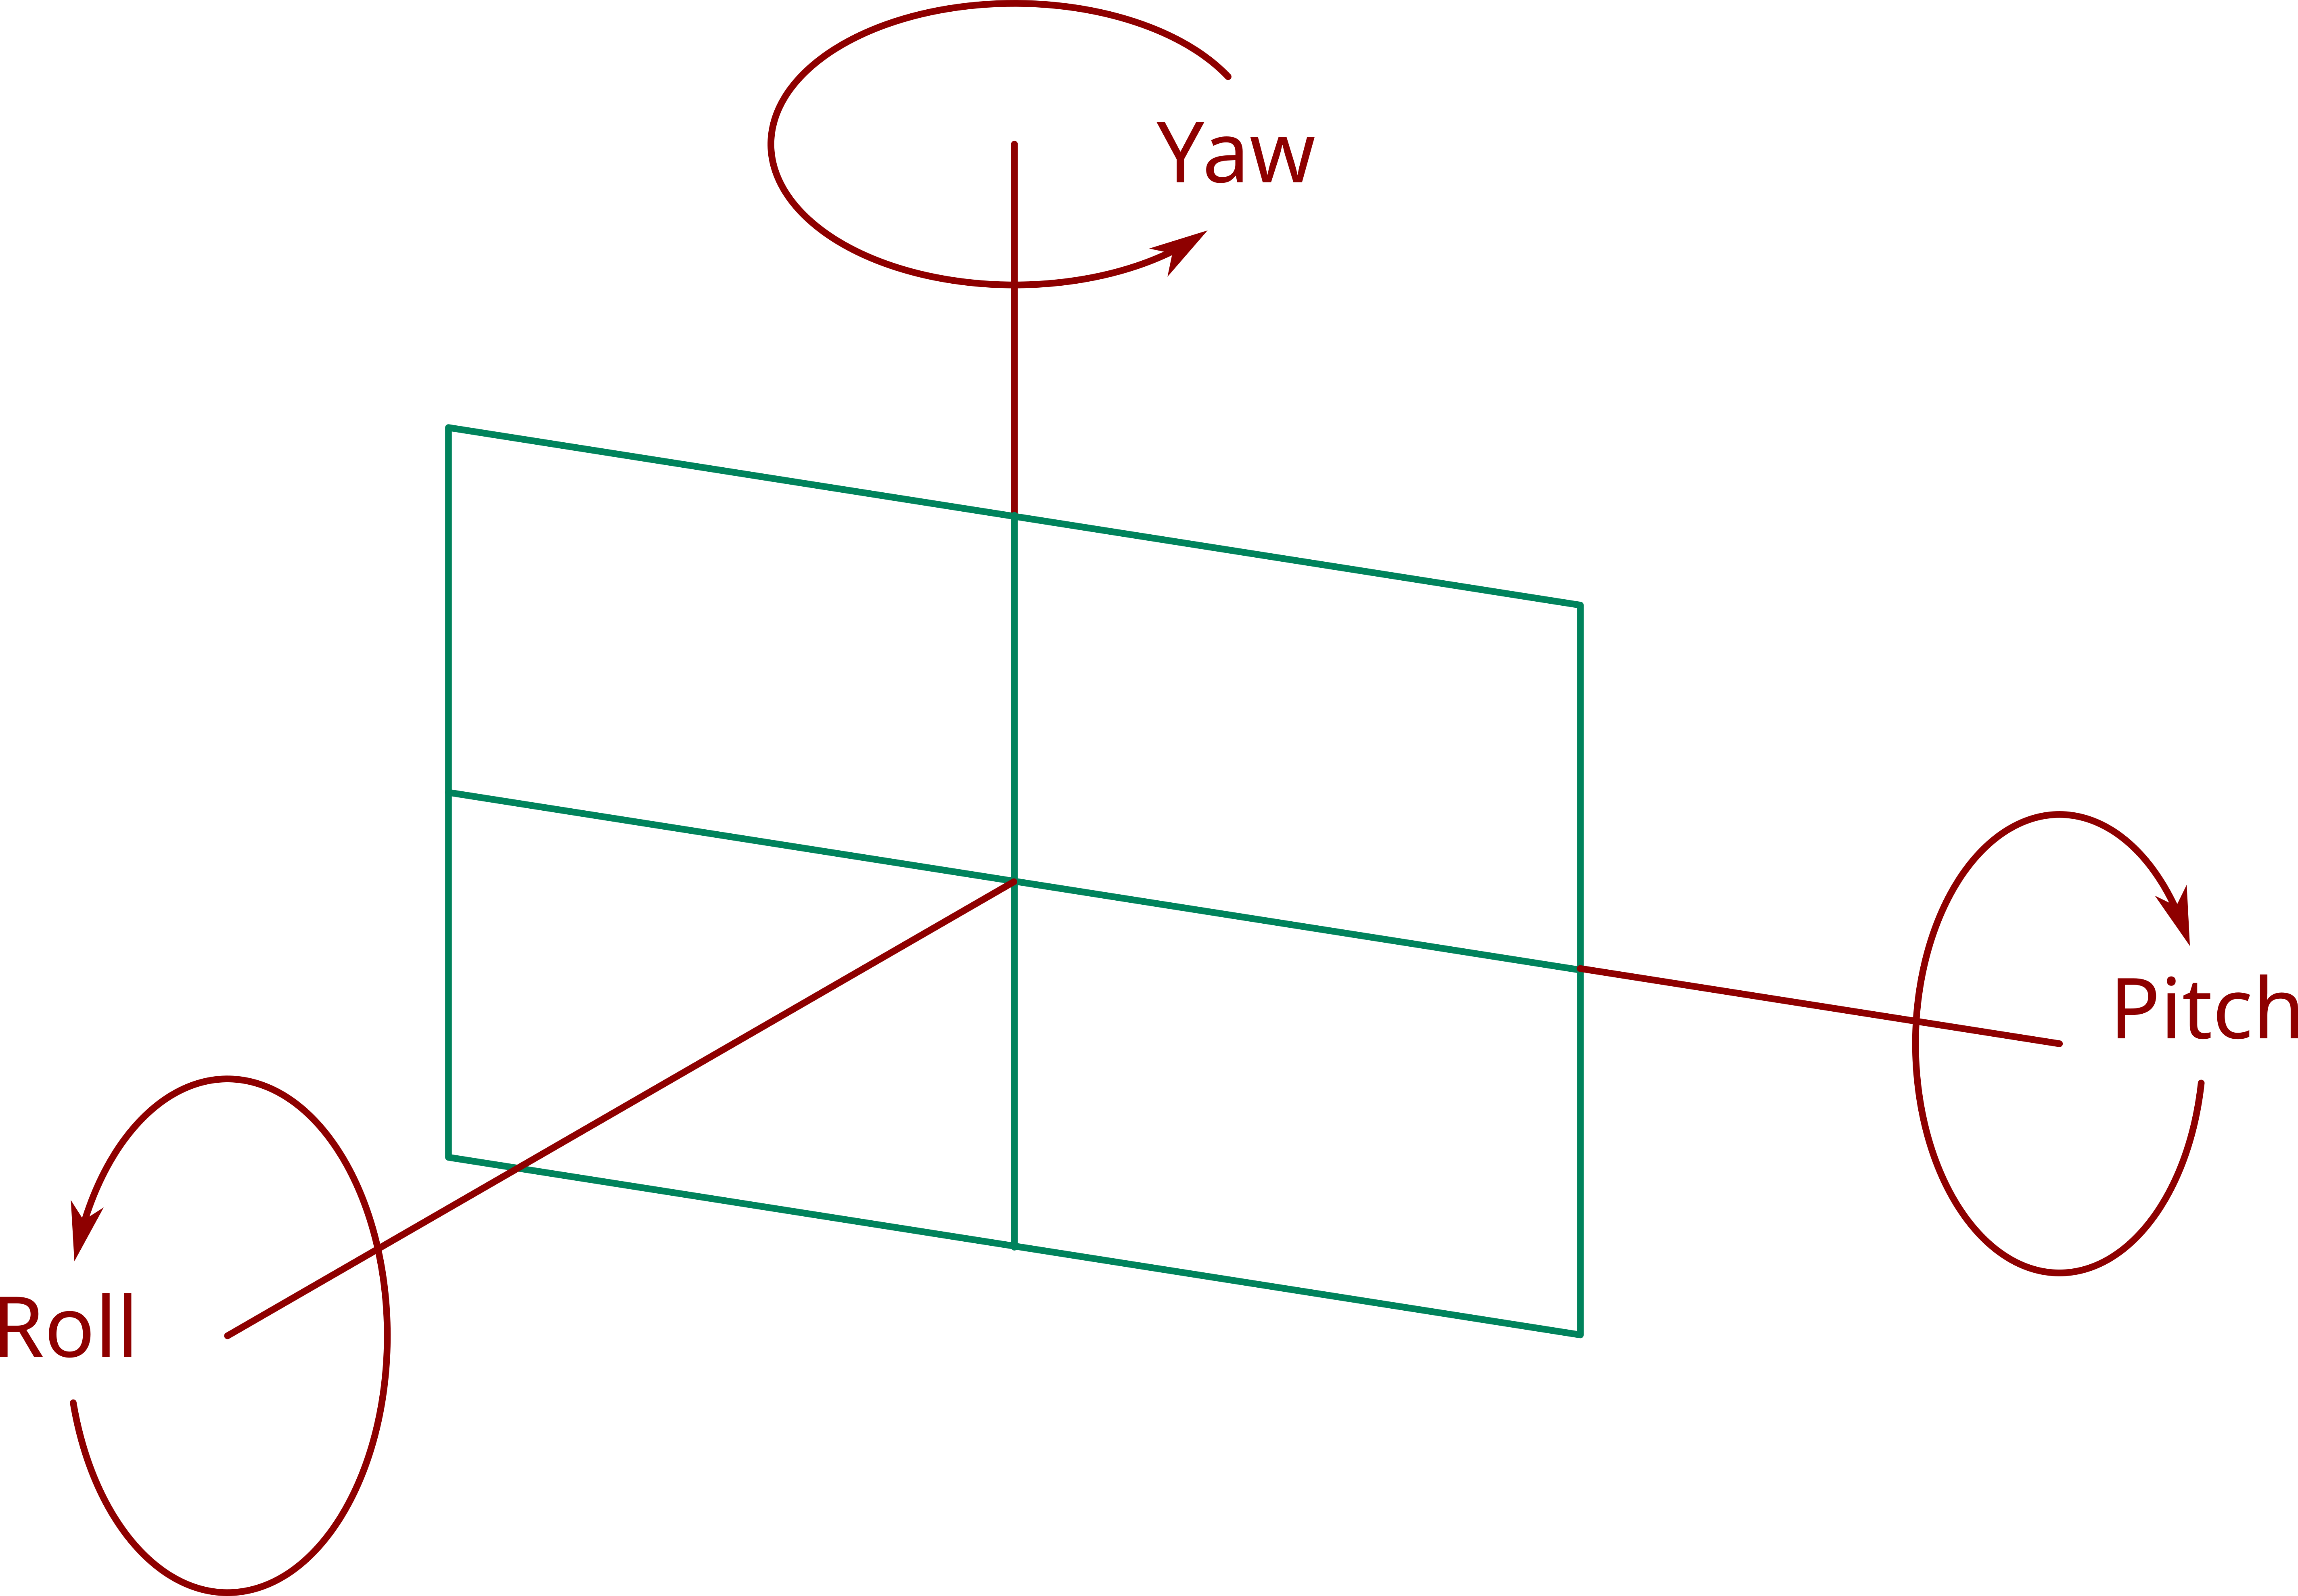
\includegraphics[width=.8\linewidth]{gfx/rollpitchyaw.png}
	\caption[Pitch, roll and yaw angles]{Pitch, roll and yaw angles}
	\label{fig:pitchrollyaw}
\end{figure}

This model let us compute the direction of the incoming rays just by indexing the particular pixel they hit, obtaining a map
\begin{equation}
	\label{eq:pixelmap}
	(p_x, p_y) \xmapsto{\mathfrak{h}_2} (\vartheta_{cs}, \varphi_{cs}),
\end{equation}
where $(p_x, p_y)$ are the components of the pixel in a system of coordinates whose origin is placed at the top-left corner of the sensor.

By composing \autoref{eq:initmap} and \autoref{eq:pixelmap}, we define the map
\begin{equation}
	(p_x, p_y) \xmapsto{\mathfrak{h} = \mathfrak{h_1}\circ\mathfrak{h_2}} (\vartheta', \varphi'),
\end{equation}
that summarises all the work the algorithm does: from a pixel on the camera's reference frame, we compute the origin of the incoming ray that hit that pixel.

\subsection{Pixel to Ray Map}
\label{subcsec:pixeltoray}

Let us consider a pixel $P$ whose coordinates on the sensor's reference frame are, in physical units, $(p_x, p_y)$, as depicted in \autoref{fig:pinhole}.

\begin{figure}[bth]
	\myfloatalign
	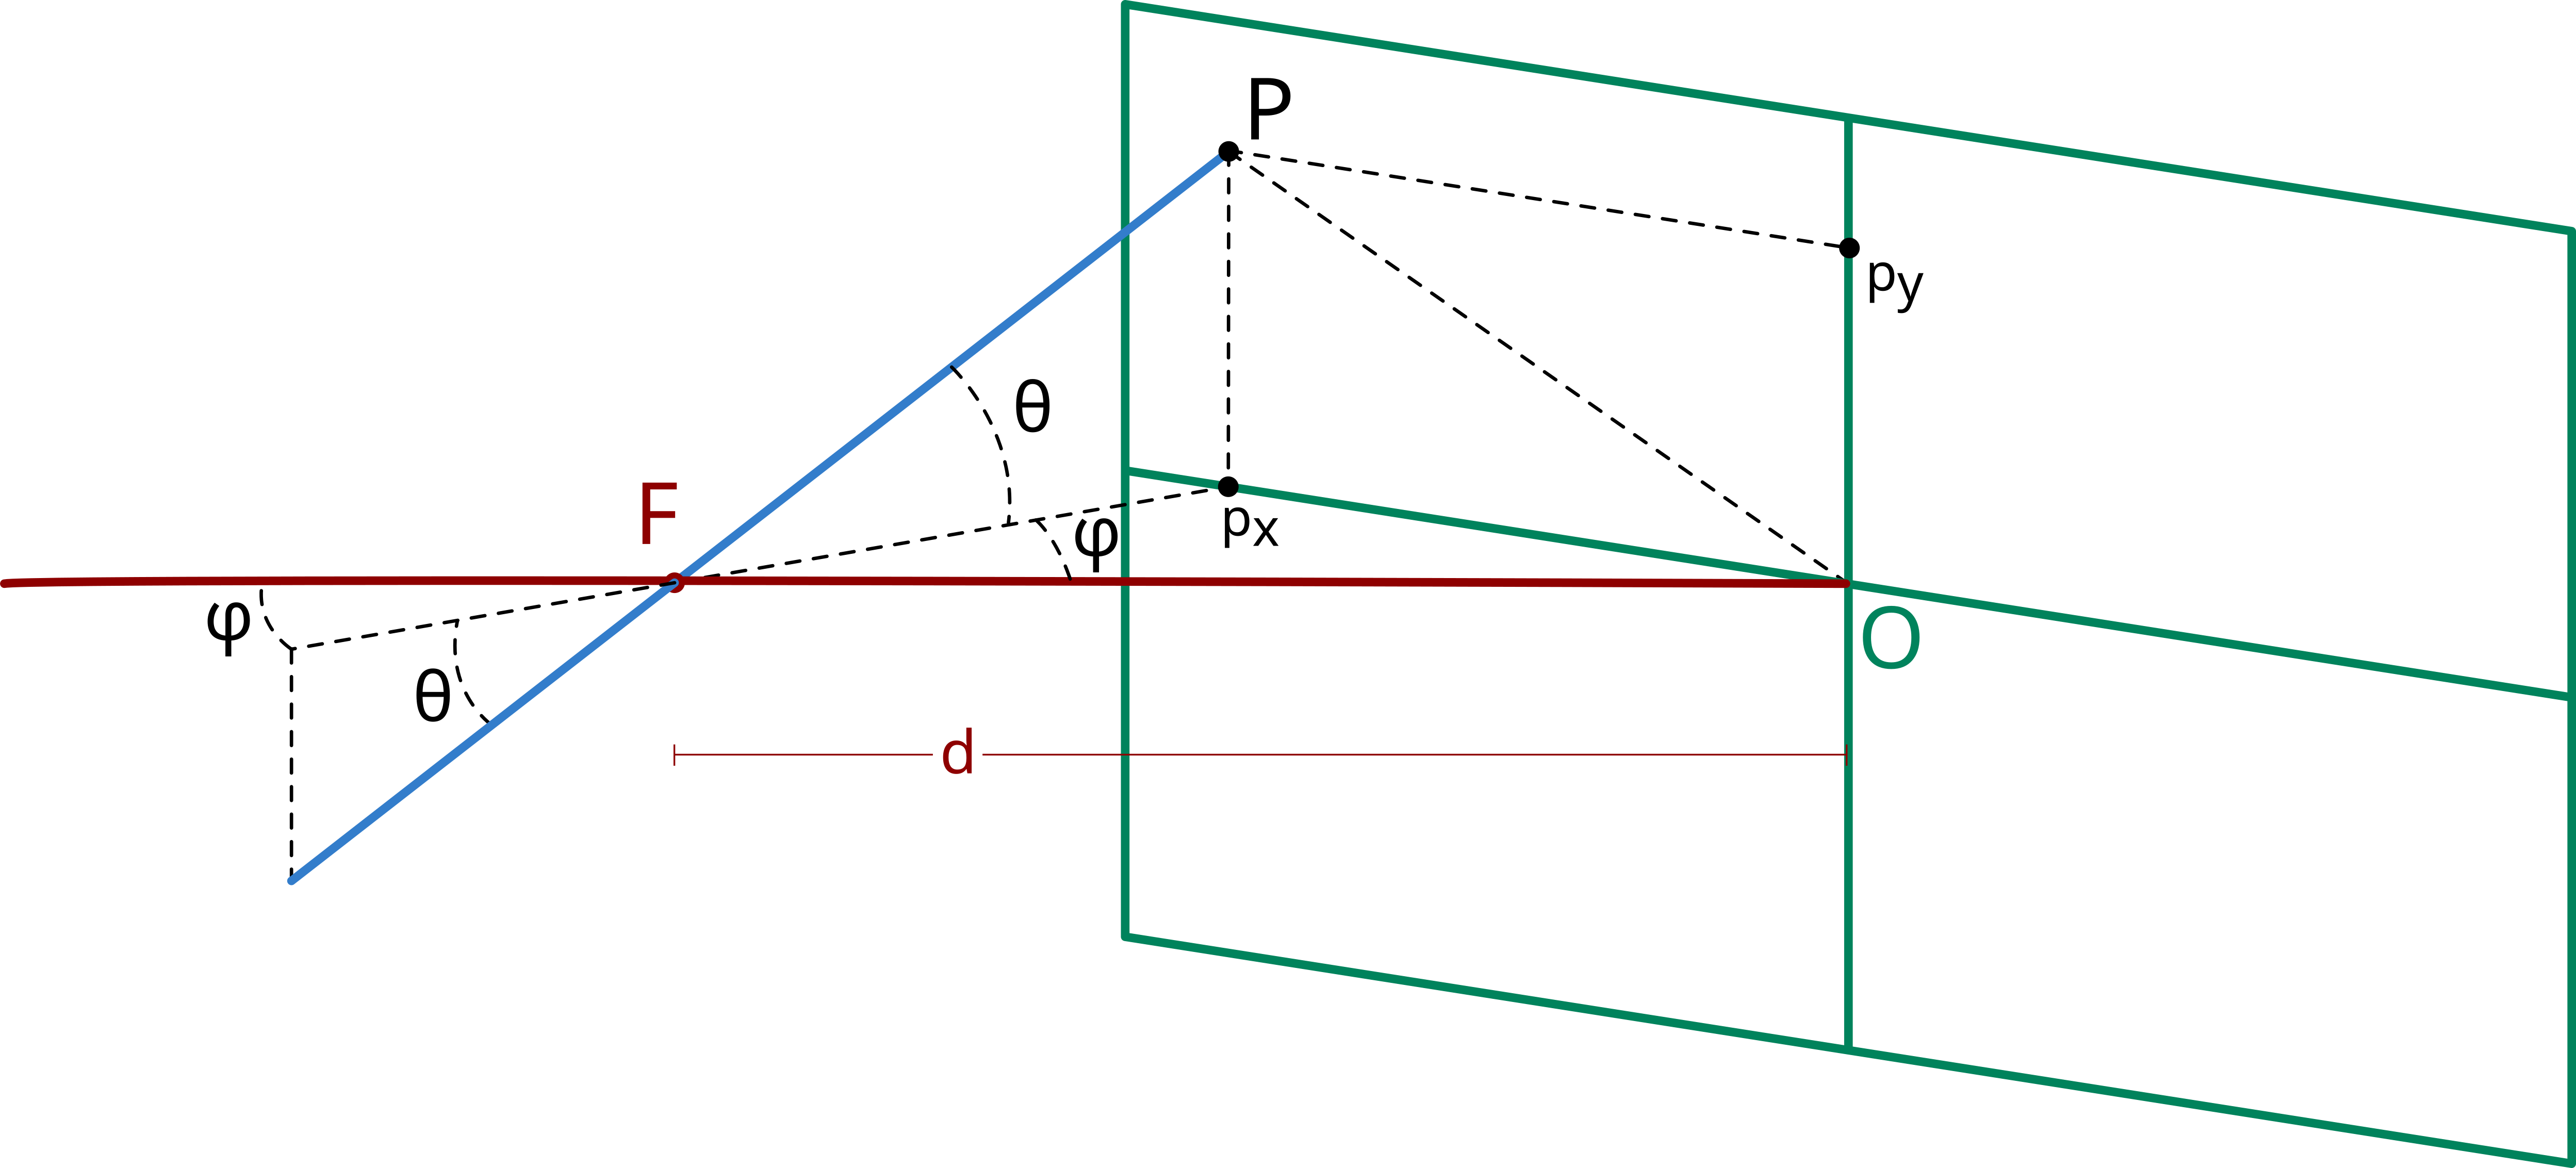
\includegraphics[width=.8\linewidth]{gfx/pinhole.png}
	\caption[Pinhole camera model]{Pinhole camera model}
	\label{fig:pinhole}
\end{figure}

All rays that hit the sensor are assumed, by our model, to pass through the focal point $F$. Thus, we can compute the angles $\vartheta$ and $\varphi$ for the ray hitting the sensor at pixel $P$ with elementary trigonometry.

From triangle $Fp_xO$ in \autoref{fig:pinhole}, we can obtain the angle $\varphi$ as
\[
	\varphi = \arctan{\frac{p_x}{d}}.
\]

Similary, the value of $\vartheta$ comes from the triangle $Fp_xP$ in \autoref{fig:pinhole}, which results in the following formula:
\[
	\vartheta = \arctan{\frac{p_y}{\sqrt{p_x^2 + d^2}}}.
\]

Finally, we need to adjust the zero for both $\vartheta$ and $\varphi$ to agree with the angle convention of the coordinate system. Therefore, the final formulas to computing the direction of an incoming ray hitting the camera's sensor ar a pixel $P = (p_x, p_y)$ are the following:
\begin{align}
	\vartheta_{cs} &= \frac{\pi}{2} + \arctan{\frac{p_y}{\sqrt{p_x^2 + d^2}}}, \\
	\varphi_{cs} &= \pi + \arctan{\frac{p_x}{d}}.
\end{align}

This discussion assumed the pixel coordinates to have its origin at the centre of the sensor. This is not the common coordinate system for pixels, as it usually have its origin at the top-left corner. A simple translation fixes that.

Furthermore, the pitch, roll and yaw angles were assumed to be zero. However, the addition of these angles is not difficult:
\begin{itemize}
	\item The roll angle, noted as $\alpha$, defines the rotation of the sensor on the image plane, so every pixel $(p_x, p_y)$ has to be rotated accordingly:
	\[
		\begin{pmatrix}
			p'_x \\
			p'_y
		\end{pmatrix} = 
		\begin{pmatrix}
			\cos\alpha & -\sin\alpha \\
			\sin\alpha & \cos\alpha 
		\end{pmatrix}
		\begin{pmatrix}
			p_x \\
			p_y
		\end{pmatrix}
	\]
	\item The pitch angle, noted as $\eta$, has to be simply added to the $\vartheta$ coordinate, as it defines the rotation of the sensor on that axis.
	\item The yaw angle, noted as $\lambda$, is the rotation of the sensor with respect to the $\varphi$ axis, so it has to be added to that coordinate.	
\end{itemize}

Taking all this into account, the final formulas to compute $(\vartheta_{cs}, \varphi_{cs})$ from the physical coordinates of the pixel $(p_x, p_y)$ are
\begin{align}
	\vartheta_{cs} &= \eta + \frac{\pi}{2} + \arctan{\frac{p_y}{\sqrt{p_x^2 + d^2}}}, \\
	\varphi_{cs} &= \lambda + \pi + \arctan{\frac{p_x}{d}}.,
\end{align}
where
\[
	p'_x = p_x\cos\alpha - p_y\sin\alpha, \qquad
	p'_y = p_x\sin\alpha + p_y\cos\alpha.
\]

\section{Initial Conditions Computation}
\label{sec:initcond}
The algorithm kernel integrates, backwards in time, an \ac{ODE} system. We already know the system we are working with, \autoref{theo:eqsmotion}, but for such a system to be uniquely solved, a set of initial conditions is needed.

That is, for each ray we need to know its components, \[(r, \vartheta, \varphi, p_r, p_\vartheta),\] at the time $\tau = 0$.

All rays hitting the camera share the same $r$, namely the position of the camera $r_c$.

In \autoref{subcsec:pixeltoray}, the initial $\vartheta_{cs}$ and $\varphi_{cs}$ for each ray were computed.

Therefore, we only need to compute the initial momentum components, $p_r$ and $p_\vartheta$, for each ray. In short, assuming we know the pixel the incoming ray is hitting and, thus, the $\vartheta_{cs}$ and $\varphi_{cs}$ components of the ray on the camera's local sky, we expect to obtain the map
\[
	(\vartheta_{cs}, \varphi_{cs}) \xmapsto{IC} (p_r, p_\vartheta).
\]

This is not a difficult task but a very delicate one, as some coordinate systems have to be taken into account and we should have a good understanding of them in order to properly compute the bases changes. A short summary of the work that follows is listed here:
\begin{enumerate}
	\item The initial position of the ray is known to be $(r_c, \vartheta_{cs}, \varphi_{cs})$. The components of the unit vector that points on the direction of motion of the camera, $B$, are noted as $(B_{\widehat{r}}, B_{\widehat{\vartheta}}, B_{\widehat{\varphi}})$, whereas its speed relative to the \ac{FIDO}, that is, the modulus of $B$, is noted as $\beta$.
	\item From $(\vartheta_{cs}, \varphi_{cs})$ we compute the unit vector in Cartesian coordinates, $N = (N_x, N_y, N_z)$, pointing to the direction of the incoming ray. This is computed on the camera's reference frame $\{e_x, e_y, e_z\}$, thus a simple change to Cartesian coordinates is needed.
	\item The relativistic aberration caused by the motion of the camera and its speed around the black hole causes the \ac{FIDO} to measure the direction of motion of the incoming ray slightly different. The Cartesian components of this derived unit vector, $n_F = (n_{F_x}, n_{F_y}, n_{F_z})$ need to be computed.
	\item Then, $n_F$ needs to be seen from the \ac{FIDO}'s orthonormal basis by means of the ligatures provided by the vector $B$ and the orthogonal relations. This gives us the components $(n_{F_{\widehat{r}}}, n_{F{\widehat{\vartheta}}}, n_{F_{\widehat{\varphi}}})$ on the basis $\{e_{\widehat{r}}, e_{\widehat{\vartheta}}, e_{\widehat{\varphi}}\}$.
	\item From $n_F$ expressed on the right coordinate system, we need to compute the covariant components of the four momentum $(p_t, p_r, p_\vartheta, p_\varphi)$, where we assume the energy to be unitary; \ie, $p_t = -E = -1$.
\end{enumerate}

\fixme{Explain more!}

\section{Numerical Solver}

Once we have the \ac{ODE} system and the initial conditions for the ray we want to solve, the final step is to numerically integrate, backwards in time, the geodesic followed by the ray.

The problem reduces then to numerically integrate an \ac{ODE} system, which is a well-known problem and widely studied in the literature.

In order to accomplish this task, the algorithm used by our ray tracer uses a classic Runge-Kutta method, along with an automated step size computation based on the estimated error of the step.

The Runge-Kutta method is based on the \texttt{DOPRI5} algorithm, described in \cite{hairer93} and \cite{hairer96}.

The automated control for the step size based on the estimated error follows the ideas in \cite[Sec. II.4, Subsec. Automatic Step Size Control]{hairer93}.

Furthermore, the step size is stabilized using the algorithm described in \cite[Sec. IV.2]{hairer96}.

\subsection{Adaptive Runge-Kutta Method}

The Runge-Kutta methods solve general initial values problems like the following one,
\begin{align*}
	\dot{y} = f(t,y) \\
	y(t_0) = y_0,
\end{align*}
where $y$ can be scalar or vector and $f$, $t_0$ and $y_0$ are known.

Given a pair $(t_n, y_n)$, the adaptive Runge-Kutta methods compute the value of the system at time $t_{n+1}$ as follows:
\begin{align*}
	y_{n+1} = y_n + h \sum_{i=1}^s b_i k_i\\
	y^*_{n+1} = y_n + h \sum_{i=1}^s b^*_i k_i,
\end{align*}

where $y_{n+1}$ is the new estimated value and $y^*_{n+1}$ is a higher order approximation that is used to estimate the error of the result, which is computed as $\vert y^*_{n+1} - y_{n+1} \vert$. In this notation, $h$ is the so-called \emph{step}, which is the amount of time the system is advanced, and the components $k_i$ are defined as follows:
\[
	k_i = f(t_n + c_ih, y_n + h\sum_{j=1}^{i-1} a_{ij} k_j).
\]

The coefficients $a_{ij}$, $b_i$, $b_i^*$ and $c_i$ define the model, and are usually arranged on what is called a Butcher's table (see \autoref{tab:generalbutcher} for a generic example).

\begin{table}[bth]
	\myfloatalign
	\begin{tabularx}{.54\textwidth}{c|ccccc}
		$0$&  & & & & \\
		$c_2$& $a_{21}$ & & & & \\
		$c_3$& $a_{31}$ & $a_{32}$ & & & \\
		$\vdots$& $\vdots$ &  & $\ddots$ & & \\
		$c_s$& $a_{s1}$  & $a_{s2}$ & $\cdots$ & $a_{s(s-1)}$ & \\ \hline
		& $b_1$ & $b_2$ & $\cdots$ & $b_{s-1}$ & $b_s$ \\ \hline
		& $b^*_1$ & $b^*_2$ & $\cdots$ & $b^*_{s-1}$ & $b^*_s$ \\
	\end{tabularx}
	\caption{Butcher's table for a generic adaptive Runge-Kutta method}
	\label{tab:generalbutcher}
\end{table}

Our system of \ac{ODE}, \autoref{theo:eqsmotion}, follows this model:
\begin{enumerate}
	\item $\dot{y} = (\dot{r}, \dot{\vartheta}, \dot{\varphi}, \dot{p}_r, \dot{p}_\vartheta)$,
	\item $f(t,y)$ is the right hand side of the equations and actually it does not depend on $t$, thus it can be written as $f(y)$.
	\item $t_0 = 0$ and $y_0 = (r_c, \vartheta_{cs}, \varphi_{cs}, p_{r}, p_{\vartheta})$ are the initial conditions computed in \autoref{sec:initcond}.
\end{enumerate}

The selected Runge-Kutta algorithm is a fourth order method with an estimation of the error based on a fifth order approximation, and whose Butcher's table is described on \autoref{tab:butcher}.

\begin{table}[bth]
	\myfloatalign
	\begin{tabularx}{.9\textwidth}{c|ccccccc}
		$0$&  & & & & & & \\
		$\frac{1}{5}$&  $\frac{1}{5}$& & & & & & \\
		$\frac{3}{10}$&  $\frac{3}{40}$&  $\frac{9}{40}$& & & & & \\
		$\frac{4}{5}$&  $\frac{44}{45}$&  $-\frac{56}{15}$&  $\frac{32}{9}$& & & & \\
		$\frac{8}{9}$&  $\frac{19372}{6561}$&  $-\frac{25360}{2187}$&  $\frac{64448}{6561}$&  $-\frac{212}{729}$& & & \\
		$1$&  $\frac{9017}{3168}$&  $-\frac{355}{33}$&  $\frac{46732}{5247}$&  $\frac{49}{176}$&  $-\frac{5103}{18656}$& & \\
		$1$&  $\frac{35}{384}$&  $0$&  $\frac{500}{1113}$&  $\frac{125}{192}$&  $-\frac{2187}{6784}$&  $\frac{11}{84}$& \\ \hline
		$y_1$&  $\frac{35}{384}$&  $0$&  $\frac{500}{1113}$&  $\frac{125}{192}$&  $-\frac{2187}{6784}$&  $\frac{11}{84}$&  $0$ \\ \hline
		$\widehat{y}_1$&  $\frac{5179}{57600}$&  $0$&  $\frac{7571}{16695}$&  $\frac{393}{640}$&  $-\frac{92097}{339200}$&  $\frac{187}{2100}$&  $\frac{1}{40}$
	\end{tabularx}
	\caption{Butcher's table for the ray tracer solver}
	\label{tab:butcher}
\end{table}

\subsection{Stabilization algorithm}

\section{Parallelization Techniques}

In general, the ray tracers are highly parallelizable, as they perform the same operations on different data.

In particular, our general relativity ray tracer is not different: it performs

\subsection{Classic Parallelization}
\subsection{General-Purpose Computing on Graphics Processing Units}